\documentclass[aps,prl,twocolumn,superscriptaddress,nofootinbib]{revtex4-1}

% the percent sign gives comments in Latex
% top line indicates this is for Physical Review, standard journal format,
% suitable for electronic submission of articles

% the line above is necessary to start any latex document.
% this is one variation that should work for most things.
% if you want double spaceing, use the following:
%
%\documentclass[prd,preprint,letterpaper]{revtex4}
%
% the "preprint" designation will make a wider line
% spacing, good for markup.
\usepackage{graphicx}  % this is the up-to-date package for all figures
\usepackage{amssymb}   % for math
\usepackage{verbatim}  % for the comment environment
\usepackage{color}
\usepackage{gensymb}
\usepackage{amsmath}

\usepackage[section]{placeins}

\usepackage{wrapfig}
\usepackage{hyperref}
\usepackage{titlesec}
\usepackage{amssymb}   % for math
\usepackage{verbatim}  % for the comment environment
\usepackage{color}
\usepackage[nodisplayskipstretch]{setspace}
\usepackage{amsmath}
\usepackage{blindtext}
%\usepackage[pdftex]{graphicx}
\usepackage[outdir=./]{epstopdf}
\usepackage[space]{grffile}
\usepackage{epsfig}
\usepackage[separate-uncertainty=true]{siunitx}
\usepackage{tikz}
\usepackage{pgfgantt}
\usepackage[english]{babel}
\usepackage[utf8]{inputenc}

\titlespacing*{\section}
{0pt}{.5\baselineskip}{.5\baselineskip}

\titlespacing*{\subsection}
{0pt}{.5\baselineskip}{.3\baselineskip}

\usepackage{footnote}

\bibliographystyle{apsrev}


% these are some custom control of the page size and margins
% \topmargin= 0.2in  % these 1st two may be needed for some computers
% \textheight=8.75in
%\textwidth=6.5in
%\oddsidemargin=0cm
%\evensidemargin=0cm

% this is where the actual document itself (rather than control statements) begins:

\begin{document}

% use a style that gives automatic headings
%\pagestyle{headings}



% the \title{} command generates a title.

% the \\ below is used to FORCE a line break in the middle of the sentence--
% otherwise latex computes it for you

\title{Nuclear Spectroscopy}


\author{\textbf{Bryan Yamashiro}}
\author{Christina Nelson}
\author{Corey Mutnik}
\author{Daichi Hiramatsu}

\affiliation{Department of Physics \& Astronomy, \\
University of Hawaii at Manoa,\\
2505 Correa Rd, Honolulu, HI, 96822, USA}





	      % \section is used to start a new one with a heading
\begin{abstract}

Three unique radioactive sources were used to find the absorption coefficients of Aluminum\,(Al) and Lead\,(Pb). Using the gamma peaks of several radioactive sources, a calibration of sodium iodide\,(NaI(T1)) scintillator was generated. The gamma peak calibration allows for conversion between channel numbers and gamma energy. Gamma energy for the Na$^{22}$ annihilation peak and photopeak, the two Co$^{60}$ photopeaks, and Cs$^{137}$ photopeak were at the channels, 309.10$\pm$0.24, 777.68$\pm$1.74, 705.79$\pm$0.58, 808.58$\pm$0.50, and 406.35$\pm$0.17, respectively. In the same order, the Compton edge energies were (0.110$\pm$0.013)\,MeV, (1.018$\pm$0.022)\,MeV, (0.884$\pm$0.019)\,MeV, and (0.427$\pm$0.016)\,MeV, with the two cobalt photopeaks sharing the same Compton edge. The aluminum absorption coefficient of for Co$^60$ is (0.34$\pm$0.02)\,cm$^{2}$/g, and Cs$^137$ is (0.46$\pm$0.01)\,cm$^{2}$/g. Comparing to the NIST values for Aluminum for approximately 2.5\,MeV, the accepted value was 0.02266. The sigma error for cobalt and cesium were 15.0$\sigma$ and 43.7$\sigma$. The absorption coefficient of Pb for the Co$^{60}$ and Cs$^{137}$ sources are (6.25$\pm$0.28)\,cm$^{2}$/g and (12.55$\pm$0.24)\,cm$^{2}$/g. Comparing to the NIST values for Lead for approximately 1.25\,MeV, the accepted value was 0.02988. The sigma error for cobalt and cesium were 22.2$\sigma$ and 52.17$\sigma$.


\end{abstract}

\maketitle    % this line is necessary to tell latex you are done with all
	      % of the stuff associated with the title, and now it can go
              % ahead and generate the title portion


\section{Background}

A driving factor of Heliophysics research deals with understanding high-energy phenomena that propagate from the Sun. Major solar events include bright bursts emitted from the solar surface called solar flares. Solar flares generate increased fluxes of gamma ray emissions towards Earth that are hazardous especially to astronauts aboard the International Space Station\,(ISS). Gamma radiation consists of high-energy photons\,\cite{1}. The Sun is able to create different elements for a wide spectrum of energies. The Reuven Ramaty High Energy Solar Spectroscopic Imager\,(RHESSI)\,\cite{2}, currently in low Earth orbit, is able to detect photon flux and the corresponding energies from 3\,keV to gamma rays at 17\,MeV with high time resolution. The nine germanium detectors, in figure \ref{figrhessi}, installed on RHESSI convert gamma rays into pulses of electrical current\,\cite{3}.
\\
\indent In this experiment we are able to emulate the concept behind the RHESSI spacecraft. Converse to the germanium detectors, our scintillator is an NaI(T1) crystal. Various sources of gamma rays will be used to see the correlations between the energy and the isotopes. Using the calibration derived from the gamma ray energies, the relevant application was to measure the effectiveness of radiation absorption shields of variant elements. The amount of absorbed radiation was dependent of thickness and the elemental composition of the shields. This small-scale laboratory experiment provided insight on shielding that may reduce the amount of radiation exposure for astronauts aboard the ISS. An understanding of material composition and the corresponding shielding efficiency may provide useful in larger-scaled missions. Information of shields that are thin, yet can block large doses of radiation, serve as an impetus to curbing hazards for future spaceflight missions.

\begin{figure}[h!]

\centerline{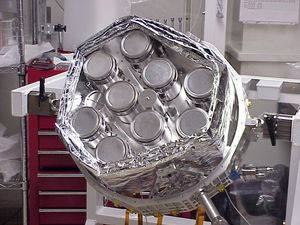
\includegraphics[width=3in]{detets.jpg}}
\caption{ \small{The nine germanium detectors installed on the RHESSI spacecraft.\,\cite{3} \label{figrhessi}}}

\end{figure}



\begin{figure}[h!]
  \begin{center}
\centerline{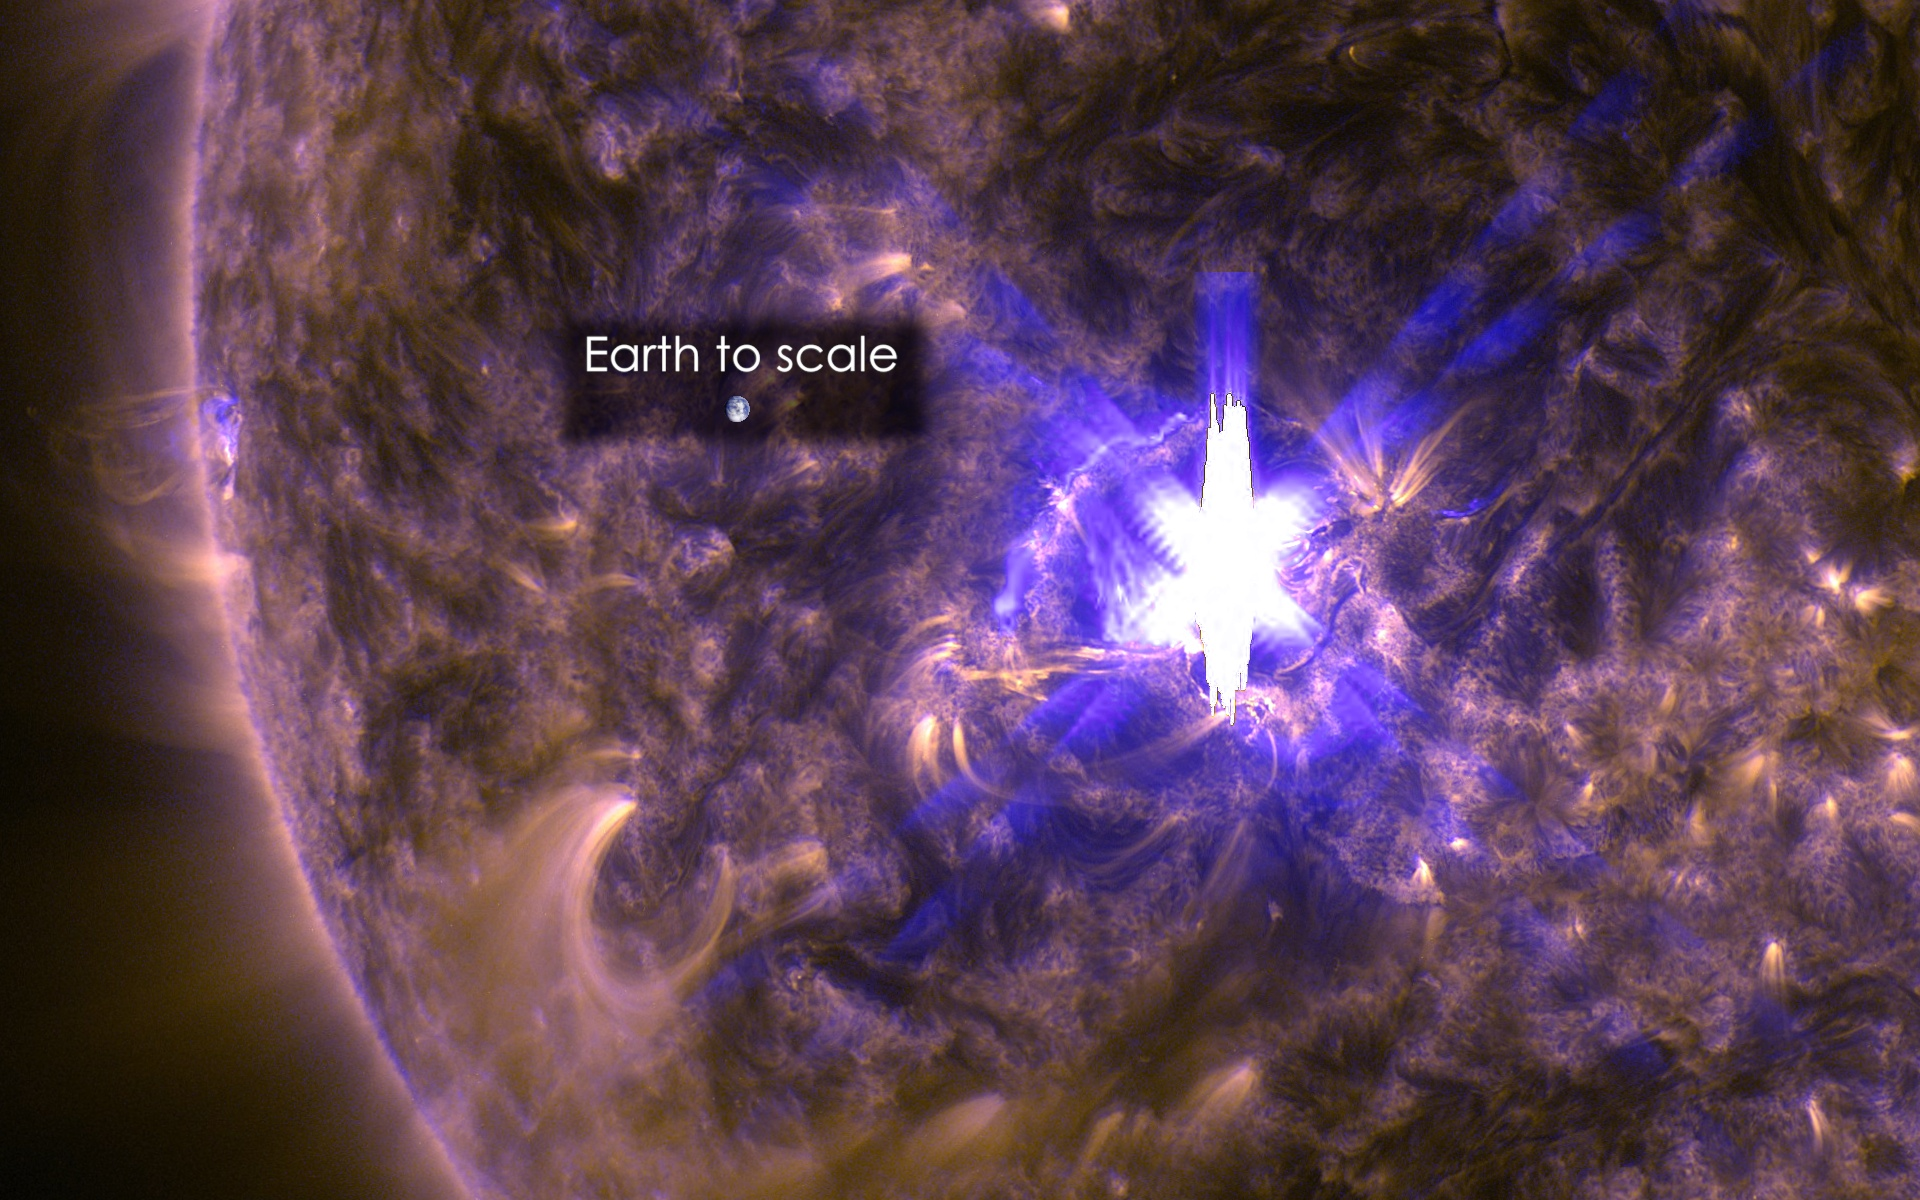
\includegraphics[width=3in]{solarflare.jpg}}
\caption{ \small{A bright and large X-class solar flare on the surface of the Sun.\,\cite{4} \label{fig1}}}
  \end{center}
\end{figure}


 % the ~\cite{ } is how you link a reference in the text. The references
 % themselves are at the end.

% one or more lines of space between paragraphs determines them

\section{Apparatus}



The nuclear spectroscopy apparatus is detailed in figure \ref{fig2}. The radioactive sources used in the experiment were Na$^{22}$, Co$^{60}$, and Cs$^{137}$. The three gamma ray sources were place in front of a Photomultiplier tube\,(PMT) equipped with a NaI(T1) scintillator. Throughout the experiment a shield of Al of Pb of varying thicknesses were placed between the source and PMT. The shields absorb a fraction of the emitted gamma rays corresponding to the respective absorption coefficients. Gamma ray flux were converted into signals of amplitude through the pre-amplifier to the Multi-Channel Analyzer\,(MCA). The MCA records the incoming signals and distinguishes the counts across 2048 channels. Finally, the computer program\,(MAESTRO) compiled the amplitude data in histograms, which could be output in ASCII format.

\begin{figure}[h!]
  \begin{center}
\centerline{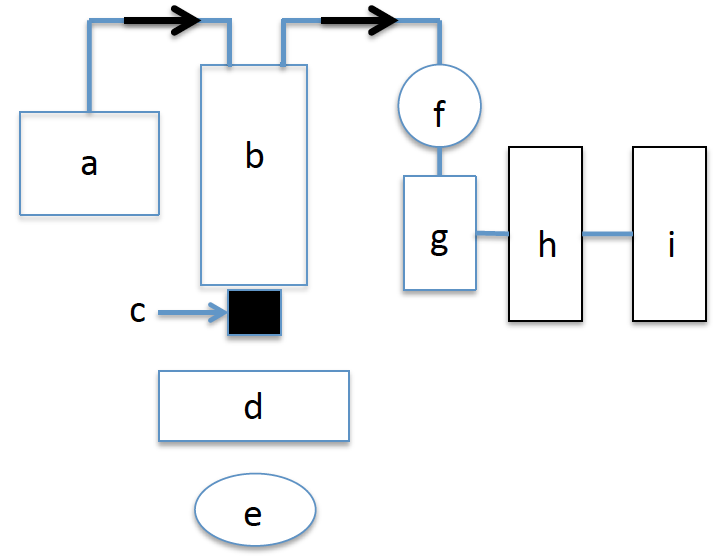
\includegraphics[width=3in]{nuke.png}}
\caption{\small{a)\,High voltage source b)\,PMT c)\,NaI(T1) Scintillator d)\,Shield e)\,Radioactive source f)\,Pre-Amplifier g)\,Amplifier h)\,MCA i)\,MAESTRO.\,\cite{5} \label{fig2}}}
  \end{center}
\end{figure}
\vspace{-.7cm}

\section{Procedure}

The experiment is separated into three parts. Initially a calibration curve was created using the apparatus without shields. A calibration curve was generated with 1) the photopeaks of the three isotopes and 2) the annihilation peak for Na$^{22}$. MAESTRO provided histograms with the MCA channel number versus gamma energy. The calibration allowed for the calculating the energy of Compton edges. The second portion of the experiment consisted of determining the fractional energy resolution $\Delta$E/E using the widths of the photopeaks and annihilation peak compared to the total energy. Finally, the absorption coefficients of the Al and Pb shields were measured. Unlike the first portion of the experiment, shields of varying thicknesses were placed between the PMT and the radioactive source. Different thicknesses were used to provide absorption data.


\vfill\eject

\section{Calculation of Results and Errors}

\subsection{Energy and Channel Number Calibration}


\begin{figure}[h!]
  \begin{center}
\centerline{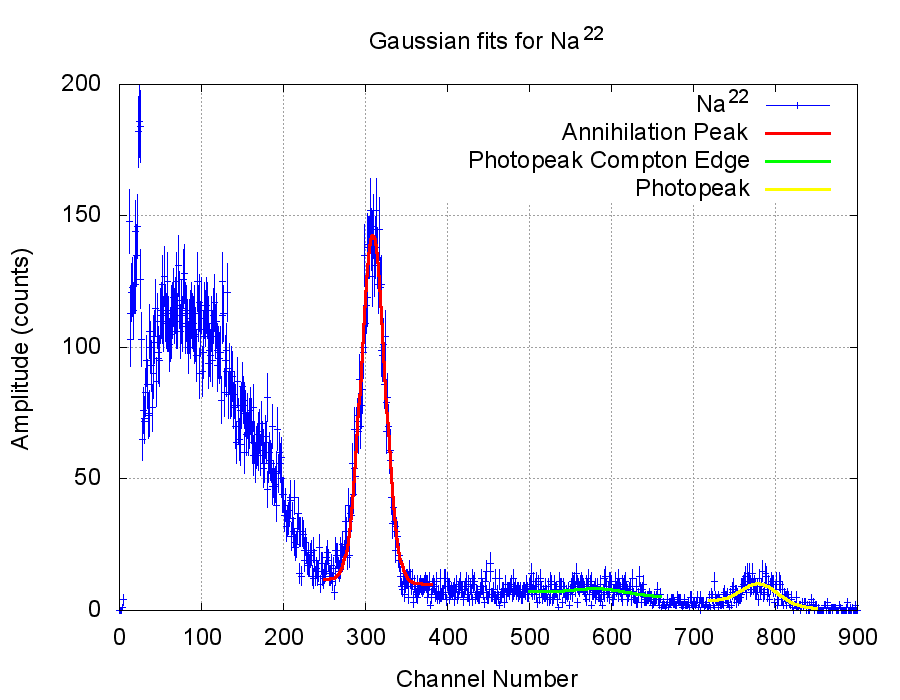
\includegraphics[width=3.5in]{nacomp.png}}
\caption{\small{A Gaussian fit on the Na$^{22}$ annihilation peak, photopeak, and photopeak Compton edge including the channel number width. The fits included a quadratic background. The unfitted peak before the annihilation peak is produced by backscatter. Due to merging between the backscatter peak and Compton edge for the annihilation peak, the annihilation Compton edge was not fit. \label{fig4}}}
  \end{center}
\end{figure}

\begin{figure}[h!]
  \begin{center}
\centerline{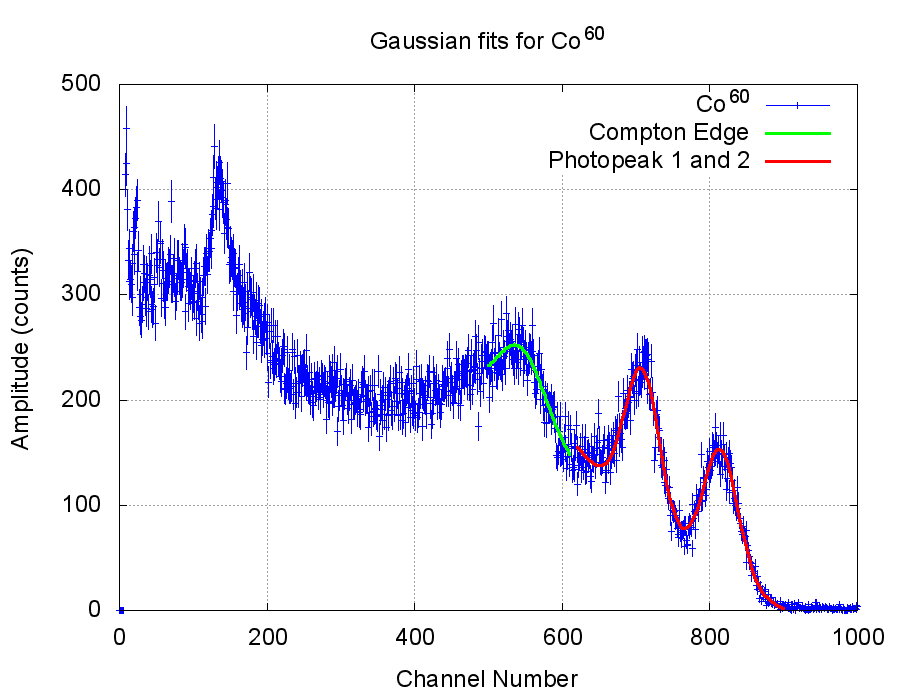
\includegraphics[width=3.5in]{cocomp.png}}
\caption{ \small{Two Gaussian fits on the Co$^{60}$ photopeak and the Compton edge of the photopeaks including the channel number width. The Gaussian fits both included quadratic backgrounds. The initial unfitted peak represents the backscatter peak. \label{fig5}}}
  \end{center}
\end{figure}
\vfill\eject
\begin{figure}[h!]
  \begin{center}
\centerline{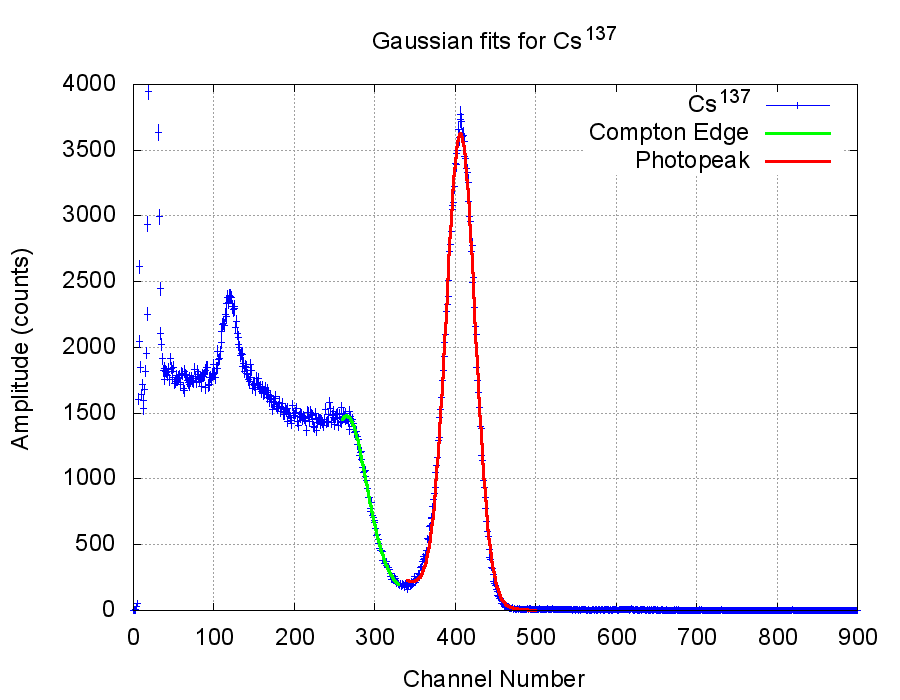
\includegraphics[width=3.5in]{cscomp.png}}
\caption{ \small{A Gaussian fit on the Cs$^{137}$ photopeak including the channel number width. The fits included quadratic backgrounds. The initial peak before the Compton edge is the backscatter peak. \label{fig6}}}
  \end{center}
\end{figure}


\begin{figure}[h!]
  \begin{center}
\centerline{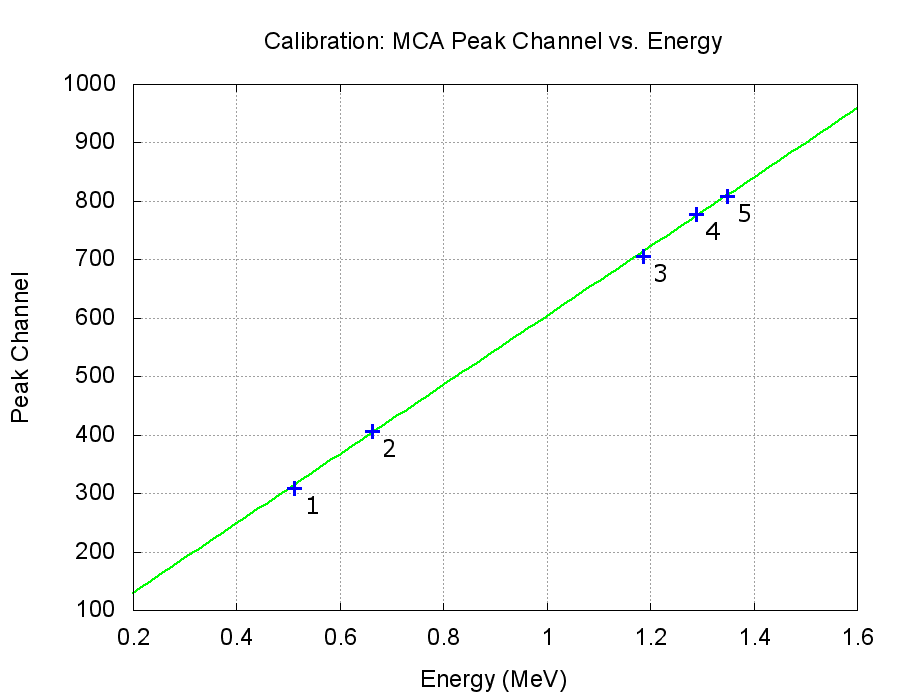
\includegraphics[width=3.5in]{calib2.png}}
\caption{\small{Linear fit calibration curve derived from the gamma peak energies for the three radioactive isotopes. 1)\,Na$^{22}$\,Annihilation Peak 2)\,Cs$^{137}$\,Photopeak 3)\,Co$^{60}$\,First Photopeak 4)\,Na$^{22}$\,Photopeak 5)\,Co$^{60}$\,Second Photopeak \label{fig3}}}
  \end{center}
\end{figure}


\begin{table}[h!] 
\caption{Gamma peak channel numbers}
 \begin{center}   % center the table on the page
    \begin{tabular}{|c|c|c|c|} \hline   % tabular environment determines the

Radioactive  & Compton Edge   & Annihilation    & \\
Isotope      &  (Channel No.)     & Peak     &  \\
             &                 &   (Channel No.)  &   \\ \hline \hline
Na$^{22}$      & - & 309.10$\pm$0.24 & - \\ \hline\hline\hline
Radioactive  & Compton Edge & Photopeak 1    & Photopeak 2 \\
Isotope      &  (Channel No.)    & (Channel No.)   & (Channel No.) \\ \hline \hline
Na$^{22}$      & 613.91$\pm$4.33 & 777.68$\pm$1.74 & - \\ \hline
Co$^{60}$      & 534.82$\pm$2.06  & 705.79$\pm$0.58 & 808.58$\pm$0.50 \\ \hline
Cs$^{137}$     & 264.37$\pm$4.78 & 406.35$\pm$0.17 & - \\ \hline
     \end{tabular}
  \end{center}
  \label{tab2}
\end{table}

\vfill\eject




\begin{table}[h!] 
\caption{Converted Compton edge energies}
 \begin{center}   % center the table on the page
    \begin{tabular}{|c|c|c|c|} \hline   % tabular environment determines the
Radioactive  & Compton  & Accepted     & Sigma \\
Isotope   &     Edge &  Value & Error \\
      &  (MeV)    & (MeV)   & (\%) \\ \hline \hline
Na$^{22}$      & 0.110$\pm$0.013 & 0.341 & 67.80 \\ \hline\hline\hline
Radioactive  & Compton  & Accepted     & Sigma \\
Isotope   &     Edge &  Value & Error \\
      &  (MeV)    & (MeV)   & ($\sigma$) \\ \hline \hline
Na$^{22}$      & 1.018$\pm$0.022 & 1.076 & 2.64 \\ \hline
Co$^{60}$      & 0.884$\pm$0.019  & 0.976 & 4.84 \\ \hline
Cs$^{137}$     & 0.427$\pm$0.016 & 0.478 & 3.19 \\ \hline
     \end{tabular}
  \end{center}
  \label{tab1}
\end{table}




\begin{equation}
E_{Compton}=E-E'
\end{equation}

\begin{equation}
E'=\frac{E}{1+\frac{2E}{0.511\,MeV}}
\end{equation}

Gaussian fits were used to pinpoint channel numbers for the gamma annihilation peak and photopeaks. A phenomena that shows up in every radioactive source graph is the backscatter peak. Backscatter peaks are created when gamma rays strike a shield and Compton scatter back into the detector, which is why the phenomena is seen at lower amplitudes and energies\,\cite{7}. Compton edges for the gamma peaks are listed in table \ref{tab2}. Equations 1 and 2 were used to obtain the accepted values of Compton energy, figure \ref{tab1}. The experimental Compton edge energies compared to the accepted energies were provided in table \ref{tab1} showing sigma errors below 5$\sigma$ for all gamma peaks. The uncertainty was propagated from the photopeak uncertainty through the calibration uncertainty. The initial photopeak uncertainty was obtained from the quadratic background Gaussian fits.
\\
\indent The Na$^{22}$ source included an annihilation peak at the channel 309$\pm$0.24 and a photopeak at 777.68$\pm$1.74. Co$^{60}$ exhibited two significant photopeaks at channels 705.78$\pm$0.58 and 808.58$\pm$0.50 for higher energies. Lastly, Cs$^137$ had a prominent photopeak at channel 406.35$\pm$0.17.
\\
\indent Figure \ref{fig3} shows the calibration curve created from each photopeak, radioactive isotope source, and annihilation peak energy of Na$^22$, and the corresponding channel numbers. The calibration curve had a slope of 591.48$\pm$12.17 with a y-intercept of (11.68$\pm$8.85)\,peak channel numbers.
\\
\indent Using the calibration curve, measured Compton edge channel numbers were converted into values of energy. The photopeak Compton edge for Na$^{22}$ was converted from channel 613.91$\pm$4.33 to (1.018$\pm$0.022)\,MeV. The channel numbers of Co$^{60}$ and Cs$^{137}$ were converted from 534.82$\pm$2.06 and 264.37$\pm$4.78 to (0.884$\pm$0.019)\,MeV and (0.427$\pm$0.016)\,MeV.




\begin{figure}[h!]
  \begin{center}
\centerline{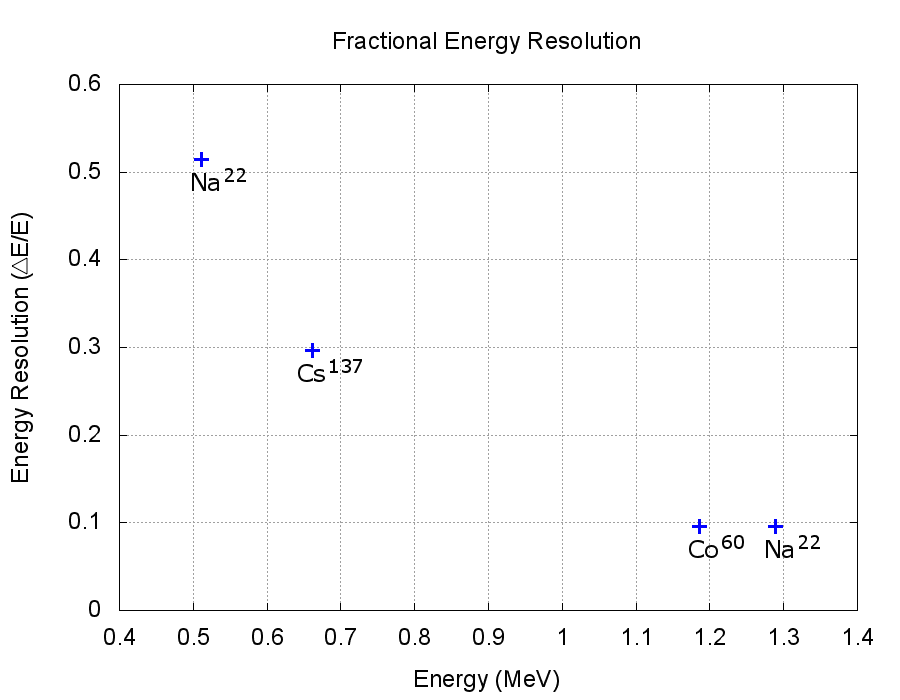
\includegraphics[width=3.5in]{frac.png}}
\caption{ \small{Energy resolution of radioactive isotopes with respective gamma peak energies. The Na$^{22}$ point furthest left represents the annihilation, and the most right Na$^{22}$ point signifies the photopeak. \label{figfrac}}}
  \end{center}
\end{figure}

A plastic scintillator has better energy resolution than an inorganic scintillator, such as NaI(T1), which is utilized in this study. Plastic scintillators demonstrate neutron responses, which allow for neutron pulses separable in liquid scintillators for higher energy resolution\,\cite{8}.
\\
\indent Using the gamma peak channel numbers and the full width half maxima of the same gamma peak, the fractional energies in figure \ref{figfrac} were found. The fractional energy resolution of the radioactive isotopes decreased as the gamma peak energies increased. At energies above 1.1\,MeV, the fractional energy seemed to taper off at approximately 0.1.
\vfill\eject
\subsection{Al and Pb Shielding}

\begin{figure}[h!]
  \begin{center}
\centerline{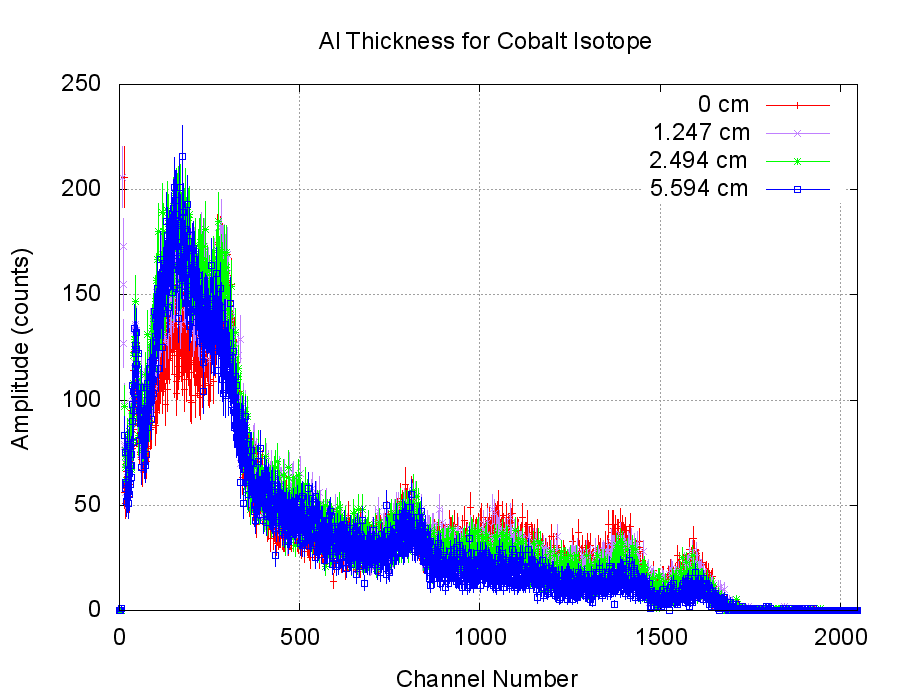
\includegraphics[width=3.5in]{cothickal.png}}
\caption{ \small{Counts of varying aluminum shield thickness for the Co$^{60}$ isotope. \label{fig7}}}
  \end{center}
\end{figure}

\begin{figure}[h!]
  \begin{center}
\centerline{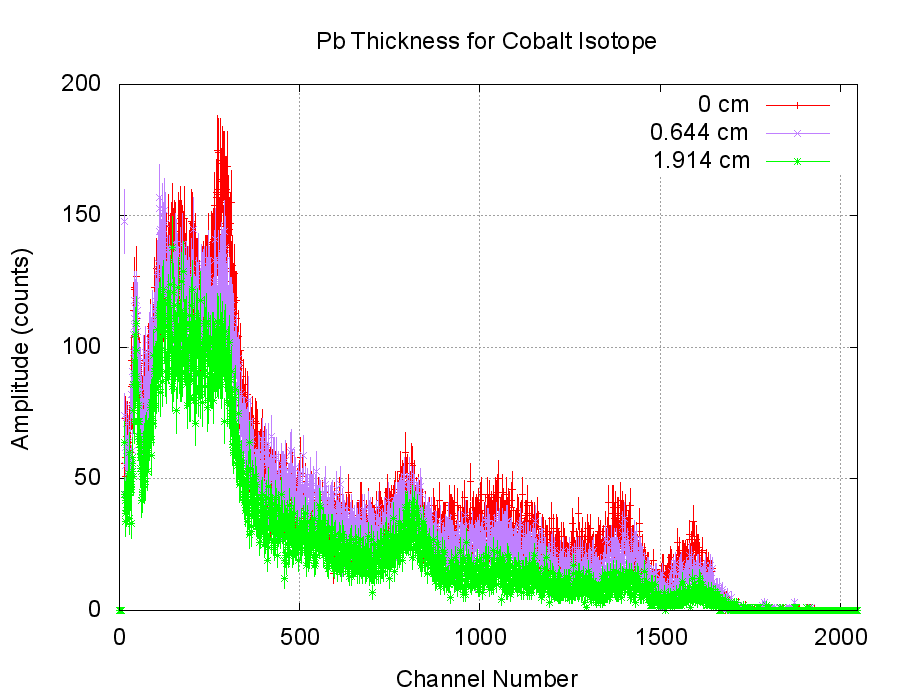
\includegraphics[width=3.5in]{cothickpb.png}}
\caption{ \small{Counts of varying lead shield thickness for the Co$^{60}$ isotope. \label{fig8}}}
  \end{center}
\end{figure}

\vfill\eject
\begin{figure}[h!]
  \begin{center}
\centerline{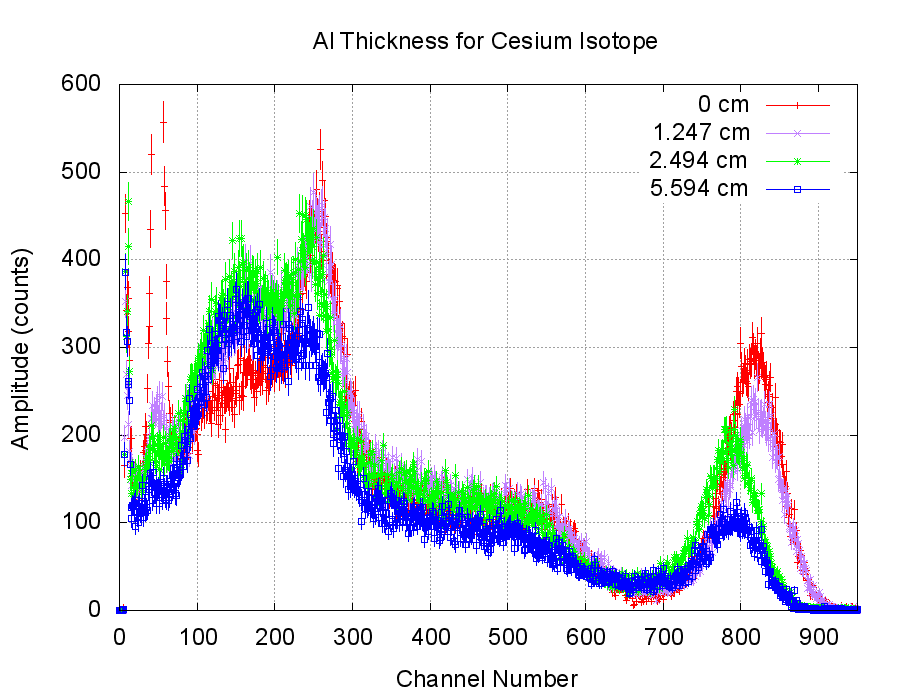
\includegraphics[width=3.5in]{csthickal.png}}
\caption{ \small{Energy spectra distributions for various aluminum shield thicknesses for the Cs$^{137}$ source. \label{fig9}}}
  \end{center}
\end{figure}

\begin{figure}[h!]
  \begin{center}
\centerline{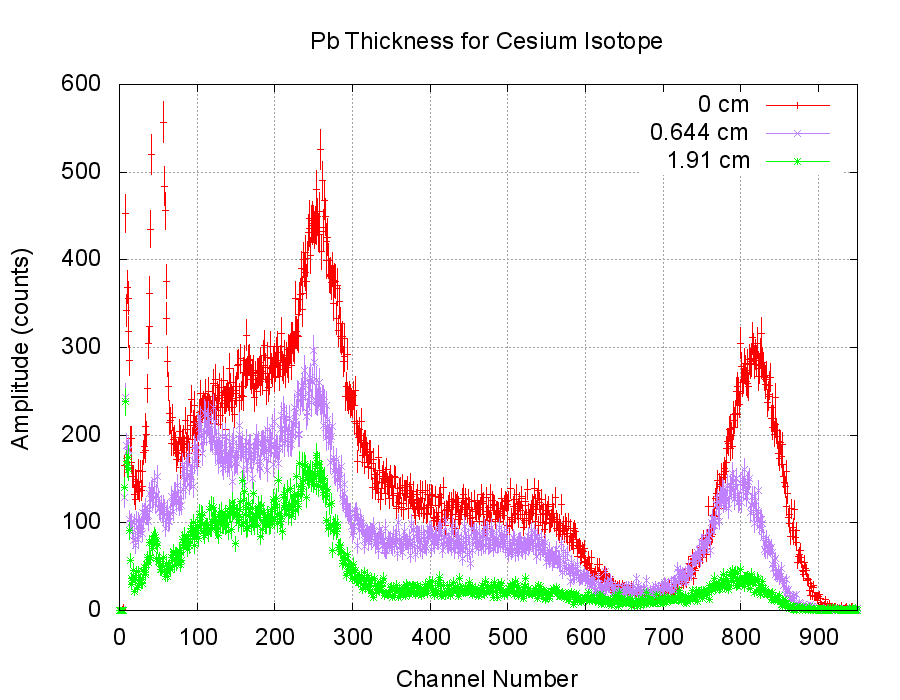
\includegraphics[width=3.5in]{csthickpb.png}}
\caption{ \small{Energy spectra distributions for various lead shield thicknesses for the Cs$^{137}$ source. \label{fig10}}}
  \end{center}
\end{figure}
\vfill\eject
\begin{figure}[h!]
  \begin{center}
\centerline{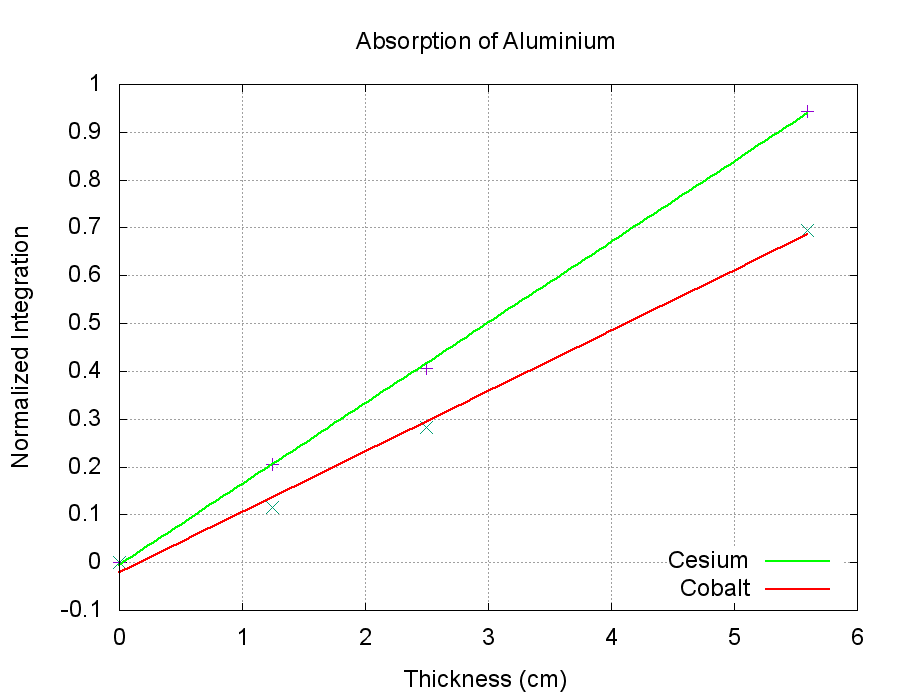
\includegraphics[width=3.5in]{muAl.png}}
\caption{ \small{Normalized integration and varying thickness for aluminum shields. \label{fig11}}}
  \end{center}
\end{figure}

\begin{figure}[h!]
  \begin{center}
\centerline{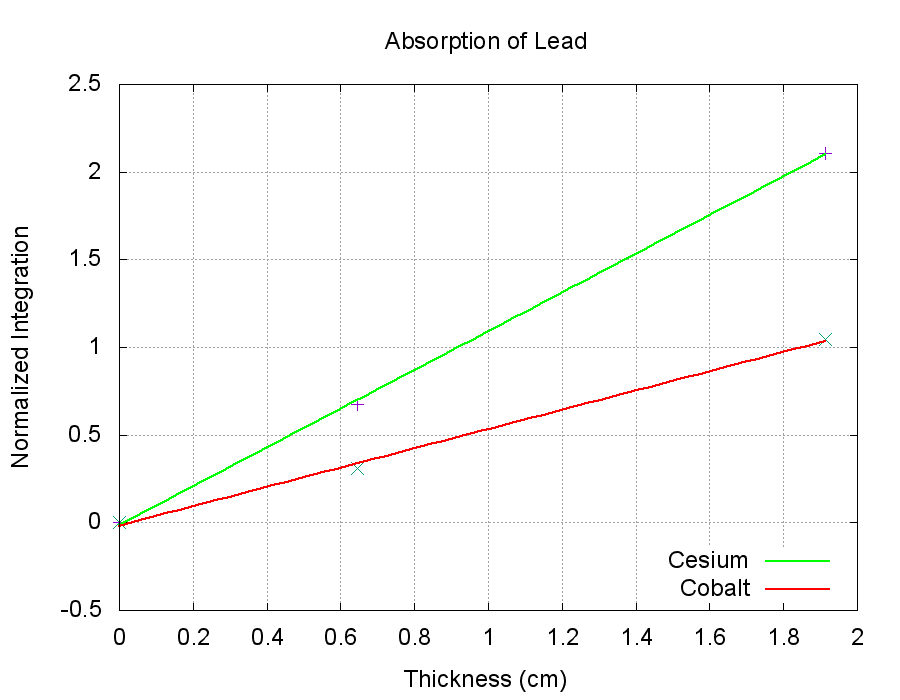
\includegraphics[width=3.5in]{muPb.png}}
\caption{ \small{Normalized integration and varying thickness for lead shields. \label{fig12}}}
  \end{center}
\end{figure}
\vfill\eject
\begin{equation}
I(x)=I(0)e^{-\mu x}
\end{equation}

Figures \ref{fig7} through \ref {fig10} showed the effect of the Al and Pb shields. Due to high absorption integration numbers, the amplitudes were normalized by the highest integration amount. As shield thickness increased, the amount of counts emitted by the radioactive source. More prominent decreases in counts were seen in the Cesium isotopes in figures \ref{fig9} and \ref{fig10}.
\\
\indent Absorptions for Al and Pb were obtained using equation 3. Equation 3 inferred  that the slope of a linear fit provided $\mu$ when I(x) was the current shield thickness count integration and I(0) was the count integration without a shield. A linear fit was traced on separate count integrations with increasing thicknesses. The slopes from the thickness fits for the Co$^{60}$ and Cs$^{137}$ sources are (0.126$\pm$0.006 and 0.169$\pm$0.002, respectively. Using the slope and the density of Al, the aluminum absorption coefficient of for Co$^60$ is (0.34$\pm$0.02)\,cm$^{2}$/g, and Cs$^137$ is (0.46$\pm$0.01)\,cm$^{2}$/g. Comparing to the NIST values for Aluminum for approximately 2.5\,MeV, the accepted value was 0.02266. The sigma error for cobalt and cesium were 15.0$\sigma$ and 43.7$\sigma$.
\\
\indent Conversely, the Co$^{60}$ and Cs$^{137}$ sources are 0.550$\pm$0.025 and 1.105$\pm$0.021. Employing the same method, the absorption coefficient of Pb for the Co$^{60}$ and Cs$^{137}$ sources are (6.25$\pm$0.28)\,cm$^{2}$/g and (12.55$\pm$0.24)\,cm$^{2}$/g. Comparing to the NIST values for Lead for approximately 1.25\,MeV, the accepted value was 0.02988. The sigma error for cobalt and cesium were 22.2$\sigma$ and 52.17$\sigma$.


\section{Discussion}

This study concludes that increases in atomic number increases the absorption coefficient of shielding. To shield from cosmic gamma rays, a heavier element shield like Bismuth would be more efficient. Weight is a major factor in space, therefore a balance between shielding elements and corresponding thickness is imperative. Gamma rays from the Na$^{22}$ source penetrated the aluminum shielding, but did not provide significant counts, therefore the correlating data was omitted.


% the following \setlength is to force the bibliography to have no
% paragraph indentations.Can use vairous units--cm are used here.
\setlength{\parindent}{0cm}

\begin{thebibliography}{99}  % the trailing 99 controls some obscure format--just use

\bibitem{1} Web. 12 Dec. 2015. \url{http://physics.nyu.edu/~physlab/Modern_2/NuclearSpec.pdf}.     % {\em } for emphasis, \textbf{ } for boldface
\bibitem{2} "National Aeronautics and Space Administration." Detectors. Web. 12 Dec. 2015. \url{http://hesperia.gsfc.nasa.gov/rhessi2/home/mission/spacecraft-instrument/detectors/}.

\bibitem{3} "H E S S I : Instrument." H E S S I : Instrument. Web. 12 Dec. 2015. \url{http://hessi.ssl.berkeley.edu/instrument/germanium.html}.

\bibitem{4} Web. 12 Dec. 2015. \url{http://www.nasa.gov/sites/default/files/thumbnails/image/20150311_x2.2_flare_earth_scale.jpg}.

\bibitem{5} "Multichannel Analyzer (MCA) Application Software." Nuclear Applications Software|ORTEC Scientific Equipment. ORTEC. Web. 5 Nov. 2015.

\bibitem{6} THE SPEED OF LIGHT. (n.d.). Retrieved November 4, 2015, from \url{http://www.phys.hawaii.edu/~teb/phys480l/SpeedOfLight.txt  http://www.phy.davidson.edu/ModernPhysicsLabs/gammaspec.html}

\bibitem{7} Web. 19 Dec. 2015. \url{http://www.phys.ufl.edu/courses/phy4803L/group_I/gamma_spec/gamspec.pdf}

\bibitem{8} Web. 19 Dec. 2015. \url{http://www.osti.gov/scitech/servlets/purl/811396/}



\end{thebibliography}





\end{document}

